\section{Abjad's object model}

\begin{frame}{Object model}
    \begin{block}
        {Abjad models musical score as a tree of components}
        Containers, leaves, spanners \& indicators
    \end{block}
    \begin{block}
        {Relationships between objects are modeled explicitly}
        Parentage, lineage, logical tie, logical voice
    \end{block}
    \begin{block}
        {Primitive objects are also modeled explicitly}
        Duration, Offset, Pitch, PitchClass, Interval, Octave, Accidental
    \end{block}
    \begin{block}
        {Top-level functions expose higher-level interfaces}
        Inspection, iteration, selection, mutation, persistence
    \end{block}
\end{frame}

\begin{frame}{Containers, leaves \& spanners}
    \begin{figure}
    \begin{centering}
        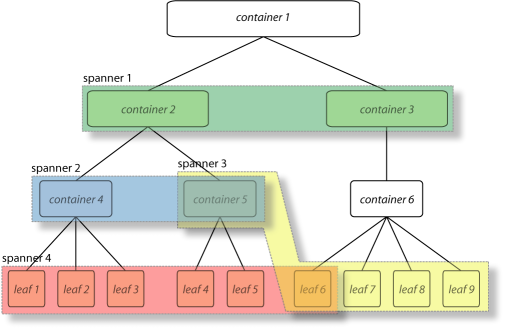
\includegraphics[height=2.5in]{assets/include-container-spanner.png}
    \caption{Spanners introducing cyclicity}
    \end{centering}
    \end{figure}
\end{frame}
